\documentclass{article}
\usepackage{graphicx} % Required for inserting images
\usepackage{fancyhdr} % Header
\usepackage{lastpage}
\usepackage[a4paper, total={6in, 8in}]{geometry}
\usepackage{float} % Floating position
\usepackage{hyperref} % Links
\usepackage{amsmath} % Math
\usepackage{amssymb} % Math
\usepackage{listings} % Import code in appendix
\usepackage{xcolor} % For coloring code
% Listing Configuration
\lstset{
    language=Python,
    basicstyle=\ttfamily\small,
    keywordstyle=\color{blue},
    stringstyle=\color{red},
    commentstyle=\color{green},
    showstringspaces=false,
    breaklines=true,
    frame=single
}
\usepackage{tikz} % Graph
\usetikzlibrary{bayesnet}
\usetikzlibrary{positioning}

\graphicspath{{images/}}

\newcommand{\authorFst}{Tristan Perrot}
\newcommand{\emailFst}{\href{mailto:tristanp@kth.se}{tristanp@kth.se}}

\pagestyle{fancy}
\fancyhf{} % clear all header and footer fields
\lhead{Assignment 1B \\ DD2434 - Machine Learning, Advanced Course}
\rhead{\authorFst}
\cfoot{\thepage \  / \pageref{LastPage}}
\setlength{\headheight}{23pt}
\setlength{\footskip}{70pt}

\title{DD2434 - Machine Learning, Advanced Course \\ Assignment 1B}
\author{\authorFst \\ \emailFst}
\date{November 2023}

\begin{document}

\maketitle

\begin{center}
  \includegraphics[scale=0.5]{KTH_logo_RGB_bla.png}
\end{center}

\thispagestyle{empty}

\newpage
\tableofcontents
\newpage

\section{CAVI for Earth quakes}

\subsection{Question 1.1}

\begin{figure}[H]
  \centering
  \begin{tikzpicture}

% Custom style for nodes without a border
    \tikzstyle{plain} = [draw=none, fill=none]

    % Define nodes
    \node[latent] (z) {$Z_n$};
    \node[plain, above=of z] (pi) {$\pi$};
    \node[latent, below left=of z] (s) {$S_n$};
    \node[latent, below right=of z] (x) {$X_n$};
    \node[latent, below=of s] (lambda) {$\lambda$};
    \node[latent, below=of x] (mu) {$\mu$};
    \node[plain, right=of x] (tau) {$\tau$};
    \node[plain, below=of lambda] (alpha) {$\alpha$};
    \node[plain, left=of alpha] (beta) {$\beta$};
    \node[plain, below=of mu] (nu) {$\nu$};
    \node[plain, left=of nu] (rho) {$\rho$};

    % Connect nodes
    \edge {pi} {z};
    \edge {z} {x, s};
    \edge {lambda} {s};
    \edge {mu} {x};
    \edge {tau} {x};
    \edge {alpha, beta} {lambda};
    \edge {nu, rho} {mu};

    % Plates
    \plate [inner sep=0.3cm] {plate1} {(z)(s)(x)} {$N$}; % Adjusted position and size
    \plate [inner xsep=0.3cm] {plate2} {(mu)(lambda)} {$K$}; % Adjusted position and size


\end{tikzpicture}

  \label{fig:fig1}
  \caption{Directed Graphical Model for the Earthquake problem}
\end{figure}

\newpage
\appendix

\section{Appendix}
\subsection{Question 1.2}\label{appendix:code.1.2}
\lstinputlisting[label = {alg:3.12}]{py_files/1.2.py}

\end{document}